% You can write any comments you want as long as there is a percentage sign at the beginning. This won't appear in your document.

\documentclass[12pt]{article}
%	options include 12pt or 11pt or 10pt
%	classes include article, report, book, letter, thesis, with 'article' being the default layout

\usepackage{amssymb,amsmath,textcomp} %These are optional packages you can install which gives you more mathematical symbols to play with

\usepackage{graphicx,subfig,enumerate,rotating} 
\graphicspath{{img/}}


%%%%%%%%%%%%%%%%%
% CUSTOM COMMANDS



%%%%%%%%%%%%%%%%%


\title{Introduction to Vision and Robotics\\Vision Practical: Coin Counter}
\author{Dylan Angus, Matthew Martin}
\date{\today}

%%%%%%%%%%%%%%%%%%%%%%%%%%%%%%%%%%%%

% OUTLINE
% Introduction
%	a paragraph outlining the task and main ideas we used to solve it
% Methods
%	for each technique we used for background subtraction
%		list their advantages and disadvantages
%		provide images of their output
%		explain why we decided to/not to use it
%	for each technique of object segmentation/separation
%		list their advantages and disadvantages
%		provide images of their output
%		explain why we decided to/not to use it
%	explain our classifier
% Results
%	provide data (e.g. confusion matrix) for how our classifier performed under testing
%	show output images from each stage of our program
% Discussion
%	discuss the success of our program, how it could be improved, challenges/limitations we faced
% Code
%	attach all matlab code that we wrote (not anything downloaded from course website)as an appendix

%%%%%%%%%%%%%%%%%%%%%%%%%%%%%%%%%%%%%

\begin{document}
	
\maketitle

\section{Introduction}

The purpose of this practical is to develop a program in Matlab that recognises and classifies several objects in an image. These objects can be coins or other small items, and the program must segment the image, identify each of the objects, and output the total value (in pounds and pence) of the objects in the image.

All of the images are taken from a downward facing camera viewing a scene containing the objects on a static background. We were provided with a set of 14 sample images on which to train our classifier (see Figure \ref{fig:samplescene} for an example).

\begin{figure}
	\centering
	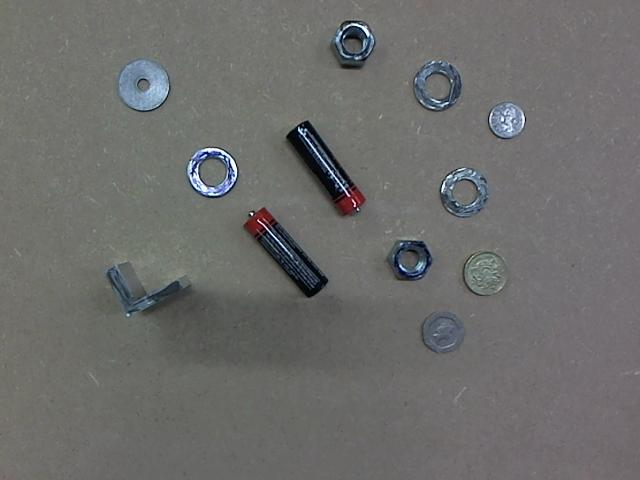
\includegraphics[width=0.75\linewidth]{02}
	\label{fig:samplescene}
	\caption{This is one of the test images given to train the classifier.}
\end{figure}

The following are the objects and associated values that may or may not be present in any given image:
\begin{itemize}
	\item one and two pound pieces
	\item 50, 20, and 5 pence pieces
	\item washer with small hole (75p)
	\item washer with large hole (25p)
	\item angle bracket (2p)
	\item AAA battery (no value)
	\item nut (no value)
\end{itemize}

We approached this problem by dividing it into three distinct stages: background segmentation, object detection, and object classification.

\section{Methods}

\subsection{Background Segmentation}

Creating a reliable algorithm that would clearly segment the background from the objects of interest in the image was the most time-consuming and challenging section of this project. We tried several different methods of background segmentation, to varying degrees of success. We ended up choosing median filter thresholding as our most successful method.

\subsubsection{Naive thresholding}

Our algorithm for creating a naive threshold can be described by the following steps:
\begin{enumerate}
	\item Attain the median values for each of the three color channels, $r,g,b$ in the given image
	\item For each pixel, if that pixel's color values are $\pm20$ from the median, label it as a background pixel. Else, label it as an object of interest.
\end{enumerate}

This method has a few advantages. It is fast, as it only requires two passes over the entire image, and there are no computationally expensive operations inside of the loop. It is simple and easy to understand. However, this method fails to accommodate for shadows in the background. It also needs to be tuned specifically to the image (the range of $\pm20$ from the medians was chosen by trial and error). Even after careful tuning, this algorithm still miss-classifies some pixels. See Figure \ref{fig:naive} for an example of the output of this method.

\subsubsection{Adaptive thresholding}

Adaptive thresholding, as opposed to naive thresholding, generates a unique threshold value for a set of sub-images inside the given image. This is meant to allow for shadows to fall on the background and still be classified as background since, the threshold is a more localized value.

This was a fairly successful method, but still had its share of disadvantages. Adaptive thresholding highlighted the edges around some of the objects rather than the objects themselves, but for others, identified the body of the object correctly. This inconsistency would cause problems when trying to classify the object. However, we never had any problems with background shadows when using this method. See the results in Figure \ref{fig:adapt}.

\subsubsection{RGB normalization}

This algorithm is meant to reduce background shadows as well by normalizing the intensity of a pixel color. It adjusts the $r,g,b$ values based on the following division:
\[r=\frac{r}{r+g+b},\hspace{5mm}g=\frac{g}{r+g+b},\hspace{5mm}b=\frac{b}{r+g+b}.\]
Then, a tight threshold can be created based on the now very similar background values. 

RGB normalization has a lot of advantages. Like adaptive thresholding, it is effective at ignoring shadows in the background. It also runs very quickly since the normalization takes advantage of Matlab's efficiency in vectorized operations, and then requires only one pass over the pixels to threshold. It produces fairly consistently good results, rarely classifying background pixels as an object. However, it often misses a couple objects in each image, which is unpredictable and would be problematic for trying to get an accurate money total for all objects in the scene. See Figure \ref{fig:norm_rgb} for an image segmented by RGB normalization.

\subsubsection{K-means clustering}

We also tried using a K-means clustering algorithm to segment the background from the foreground. This algorithm is meant to cluster all of the background pixels into the same class and then cluster all of the objects into the same class.

We saw limited success using this strategy, as it often fails to classify shadows in the background as part of the background. It is also fairly slow, as it has to run for several iterations before the clusters converge. See the results from this method in Figure \ref{fig:kmeans}.

\subsubsection{Mean-shift segmentation}

Mean-shift segmentation is a commonly recommended method for background subtraction, because, like adaptive thresholding, it localizes its segmentation to subsets of the pixels in the image. The algorithm searches for local maxima in the data and identifies that as an approximate for the background.

The performance of this algorithm varies tremendously throughout different testing images. In some images, it separates out the background almost perfectly, while in other images (see Figure \ref{fig:mean_shift}) it localizes the maximum as a background shadow, and classifies the shadow as the background. It is also a time consuming algorithm. Ultimately, we could not reduce the inconsistency in performance.

\subsubsection{Median filter thresholding}

Median filter thresholding involves using the entire dataset of images for background segmentation. This algorithm calculates the median $r,g,b$ values for each pixel throughout all of the images in the set. Then we are able to compute a pixel-by-pixel threshold for the image being segmented. We knew that the median $r,g,b$ values would correspond to the background color for that pixel location, so we put a threshold on the sum of the absolute values of the differences between the median $r,g,b$ value at a pixel and the actual $r,g,b$ value at that pixel. Here is the threshold represented mathematically, for a single pixel and a threshold $T$:
\[abs(r_{median}-r)+abs(g_{median}-g)+abs(b_{median}-b)<T\]

This algorithm consistently performed very well. It ran fairly quickly, especially after taking advantage of Matlab's vector operation optimizations. It always classified background shadows as part of the background, and usually found most of each object. We decided to use this method for our background segmentation algorithm. See Figure \ref{fig:median} for a sample output image.

\begin{figure}
	
	\centering
	\subfloat[naive thresholding] {
		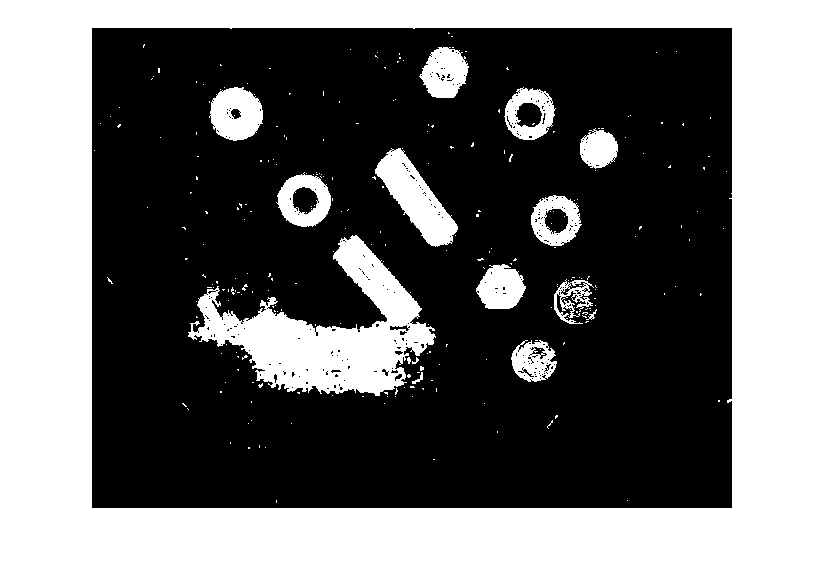
\includegraphics[width=0.5\linewidth]{naive}
		\label{fig:naive}
	}
	\subfloat[adaptive thresholding] {
		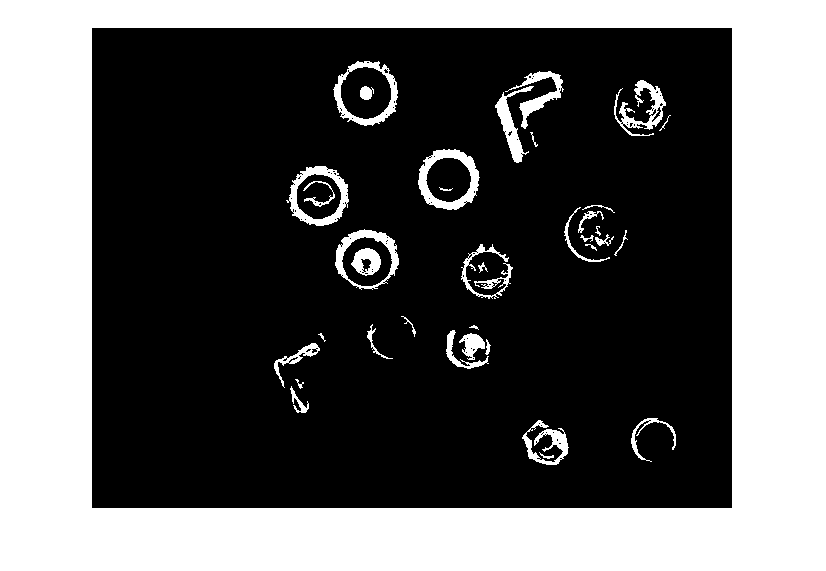
\includegraphics[width=0.5\linewidth]{adapt}
		\label{fig:adapt}
	}
	\hspace{0mm}
	\subfloat[RGB normalization] {
		
\includegraphics[width=0.5\linewidth]{norm_rgb}
		\label{fig:norm_rgb}
	}
	\subfloat[k-means classification] {
		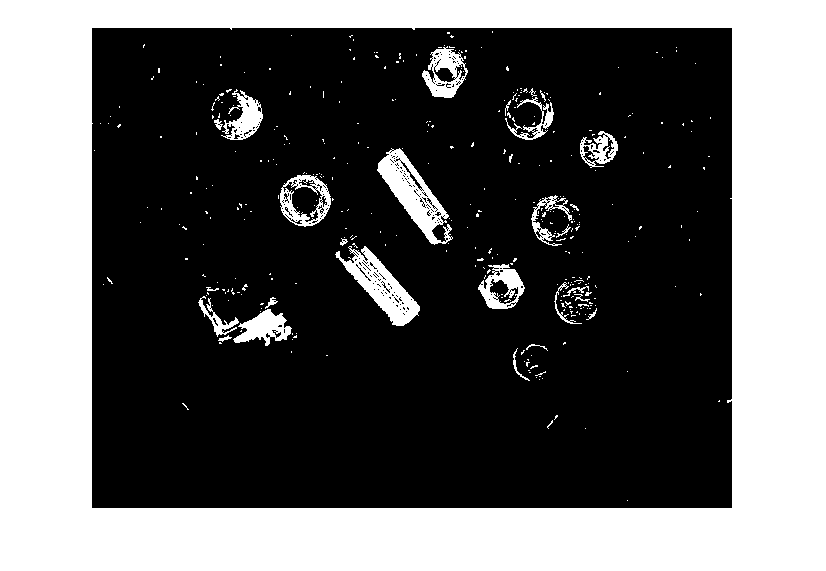
\includegraphics[width=0.5\linewidth]{kmeans}
		\label{fig:kmeans}
	}
	\hspace{0mm}
	\subfloat[mean-shift segmentation] {
		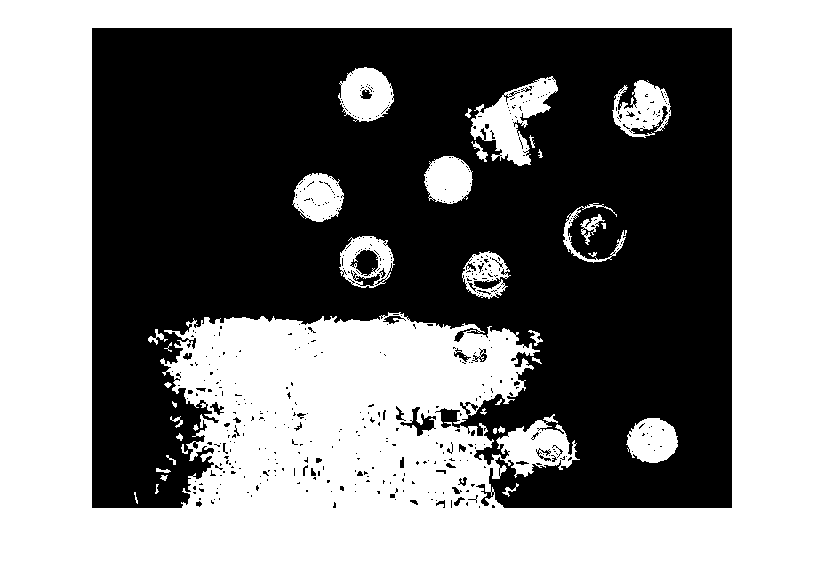
\includegraphics[width=0.5\linewidth]{mean_shift2}
		\label{fig:mean_shift}
	}
	\subfloat[median filter thresholding] {
		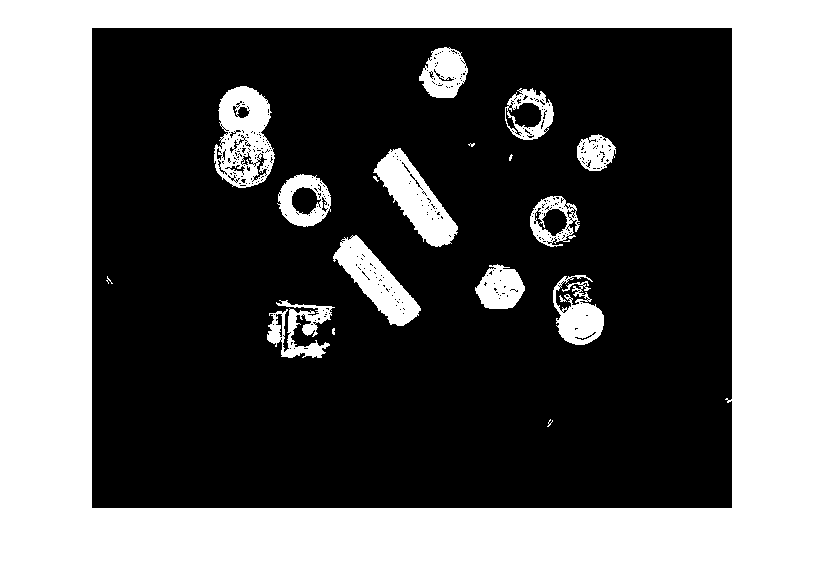
\includegraphics[width=0.5\linewidth]{median1}
		\label{fig:median}
	}
	
	\label{fig:bgseg}
	\caption{Here are the output images for the six methods of background segmentation that we tried.}
	
\end{figure}

\subsection{Object Detection}

We tried a couple different methods for detecting each object from the segmented image. The success of these methods is largely dependent on how well the background is separated from the original image. We settled on detecting boundaries in the image as the most reliable method to recognise discrete objects in the segmented image.

\subsubsection{K-means clustering}

We attempted to use k-means clustering in order to separate out the different objects in the image. The idea was to have each cluster correspond to an object in the image. However, we realized that this would not be practical to use generally because the k-means algorithm requires the number of clusters as a parameter. Since we do not know how many objects are in each image before processing it, we do not have this information for the classifier.

\subsubsection{Boundary detection}

Boundary detection works extremely well to separate out each object. The only issue is that sometimes the background segmentation breaks up an object into a few pieces. We solved this problem by doing some pre-processing on the image before passing it to the boundary detector. The pre-processing algorithm is structured as follows:
\begin{itemize}
	\item For each pixel in the image:
	\item If the pixel is white (part of an object), and the pixel that is 10 rows below it is also white, then connect the two pixels
\end{itemize}
This algorithm effectively joins up objects that are meant to be together, thus making it so they share a boundary. This image is then passed into a boundary detector, and then we return a logical matrix that is 3-dimensional: rows, columns, and a layer for each object in the image. See Figure \ref{fig:bound} for the output of this process.

\begin{figure}
	\centering
	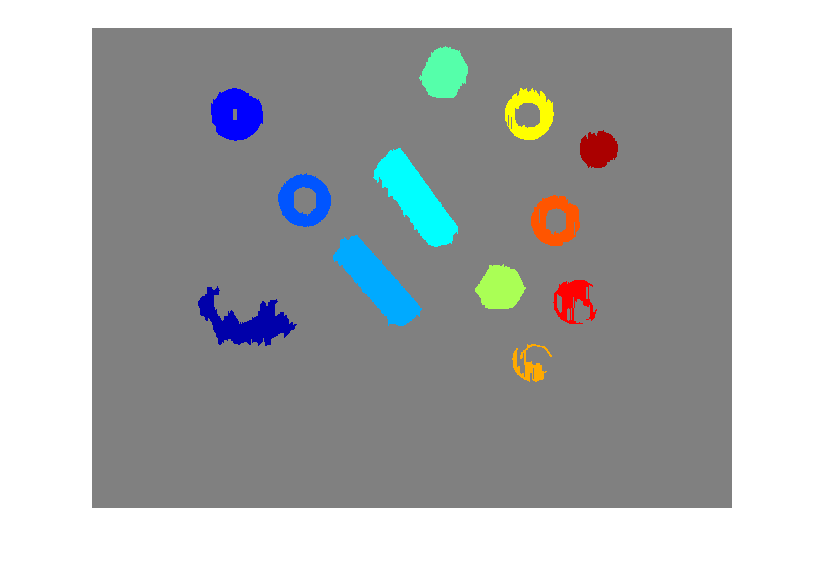
\includegraphics[width=0.8\linewidth]{boundary}
	\caption{Here is an image after background subtraction and boundary detection. Each color corresponds to a unique object as identified by its boundary.}
	\label{fig:bound}
\end{figure}

\subsection{Classification}

The classification process consisted of two main parts: feature selection and classifier training.

\subsubsection{Feature selection}

Feature selection is an extremely important stage in claification. Choosing features that allow the classifier to make clear distinctions between different objects in the image is essential to the success of the classifier. We chose to extract the following features from each object in the image for our classifier:

\begin{itemize}
	\item Mean $r,g,b$ values
	\item 1 complex moment (ci1)
	%\item SURF features
	\item Compactness
\end{itemize}

These features were calculated given a subimage of the overall image that contains only the object of interest. See Figure \ref{fig:5pencesub} for an example of a 5 pence piece that would be analyzed for these features.

The process of deciding to use this feature set relied on trial and error. We attempted several other combinations as well, but achieved worse results as compared to the accuracy of these features. We tried to use simply mean $r,g,b$ values and 6 complex moments. In this instance, the extra several complex moments did not seem to improve performance, so we eliminated them. We tried adding in major axis length and minor axis length, however, this was only useful in separating out the batteries and angle brackets, which were already being classified fairly accurately. We then tried integrating SURF and FAST features into the analysis, but the low resolution of the segmented objects caused these features to have a very little influence on the overall classification. Further, the acquisition of these two features took longer than any others, so the extra computation time did not justify the minimal/lack of a benefit. It turned out that keeping the features as concise as possible yielded the best results.

\begin{figure}
	\centering
	
\includegraphics[width=0.5\linewidth]{subimage}
	\caption{A five pence piece extracted from a training image.}
	\label{fig:5pencesub}
\end{figure}

\subsubsection{Classifier training}

Upon testing the multivariate gaussian classifier with all the features in the feature vector grouped together, we realized that there was not enough training data to properly approximate the covariance matrix. Thus, we then chose to approximate the distribution by using a Naive Bayes classifier instead. By assuming independence between the group of RGB means and group containing the compactness and c1 moment together, we used a multivariate gaussian distribution to approximate each of their conditional distributions and then found the class which maximised the product of their conditional probabilities and prior probabilities of the classes. Doing this the performance rose drastically.

\section{Results}

In order to assess the accuracy of our classification model, we split the data into a training and a testing set, giving 75\% to training and 25\% to testing. We calculated $precision$, $recall$, and $F_1$ values for each class. These two measures are widely used to assess the performance of classification models and are calculated as follows (where $tp=TruePositives,fp=FalsePositives,fn=FalseNegatives$):

\[precision=\frac{tp}{tp+fp},\hspace{5mm}recall=\frac{tp}{tp+fn},\hspace{5mm}F_1=\frac{precision*recall}{precision+recall}\]

We calculated average precision and recall across each of the ten classes in the testing data and achieved the following results: 

\[precision=0.739,\]
\[recall=0.731,\]
\[F_1=0.715.\]

We generated a confusion matrix from our testing data. This can be seen in Table \ref{tab:conf}. Figure \ref{fig:pipeline} shows the output of our program at each stage of the process, as described in the Methods section.

\begin{sidewaystable}[]
	\centering
	\caption{Confusion matrix for data from testing classification. Zeros were omitted for readability.}
	\label{tab:conf}
	\begin{tabular}{l|l|l|l|l|l|l|l|l|l|l|l}
					& AAA & aBracket & 50p & 5p & Nut & 1Pound & 20p & 2Pound & WashLgHole & WashSmHole & NotSure \\ \hline
		AAA 		& 2   &          &     & 	&     & 	   &     &        &            &            & 		  \\ \hline
		aBracket 	&     & 2        &     &  	&     & 	   &     &        &            &            &		  \\ \hline
		50p 		&     &          & 1   & 	&     & 	   & 1   &        &            &            &		  \\ \hline
		5p 			&     &          & 1   & 3	&     & 	   &     &        &            &            &		  \\ \hline
		Nut 		&     &      	 &     & 	& 2   & 	   &     &        &            &            &		  \\ \hline
		1Pound 		&     & 		 &     & 	&     & 2	   &     &        &            &            &		  \\ \hline
		20p		 	&     & 1		 &     & 	&     & 	   & 2   &        & 1          &            & 1		  \\ \hline
		2Pound 		&     & 		 &     & 	&     & 	   & 1   & 2      &            & 1          &		  \\ \hline
		WashLgHole 	&     & 		 &     & 	&     & 	   & 1   &        & 8          &            &		  \\ \hline
		WashSmHole 	&     & 		 &     & 	& 2   & 	   &     &        &            & 3          &		  \\ \hline
		NotSure 	&     & 		 &     & 	&     & 	   &     &        &            &            &		  
	\end{tabular}
\end{sidewaystable}

\begin{figure}
	\centering
	\subfloat[original image] {
		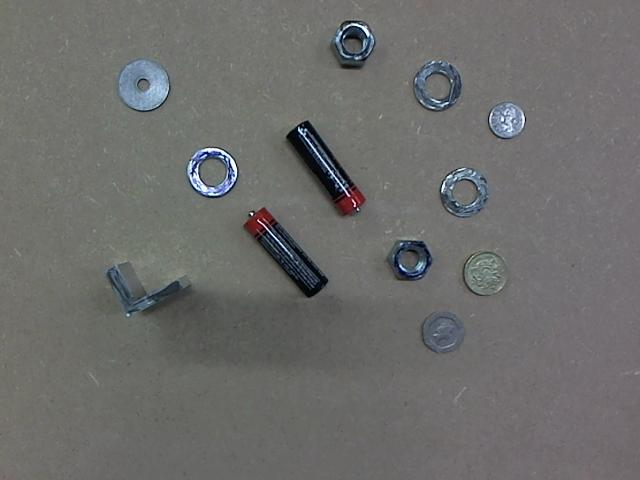
\includegraphics[width=0.32\linewidth]{02}
	}
	\subfloat[background segmented] {
		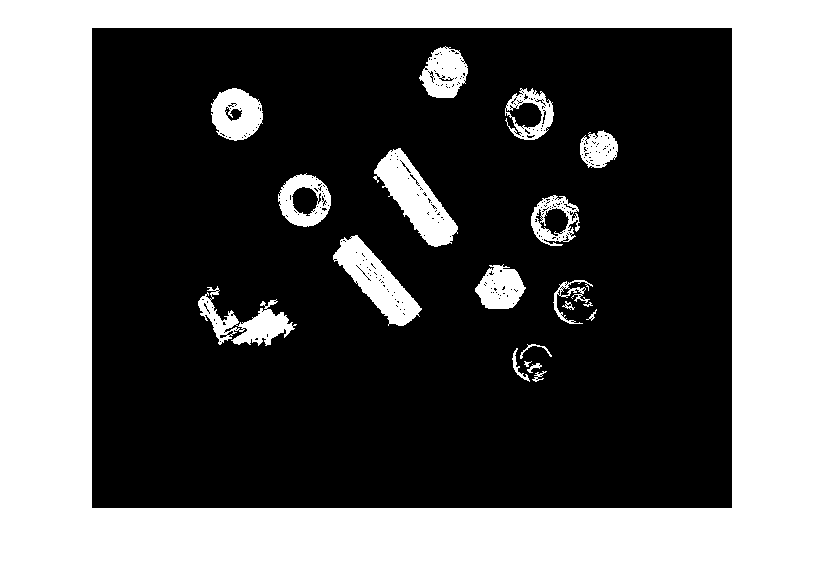
\includegraphics[width=0.38\linewidth]{median02}
	}
	\subfloat[object extraction] {
		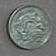
\includegraphics[width=0.3\linewidth]{1pound}
	}
	\hfill
	\subfloat[classification] {
		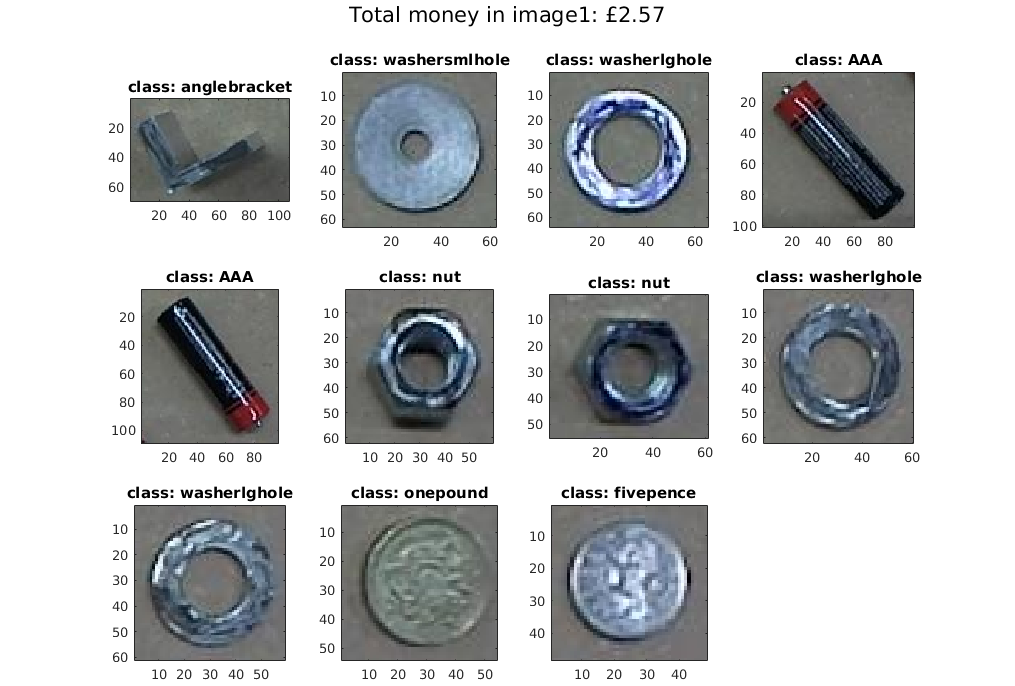
\includegraphics[width=\linewidth]{classified02}
	}
	\caption{This shows the overall pipeline of our program. The original image is segmented, objects are extracted, and then classified.}
	\label{fig:pipeline}
\end{figure}


\section{Discussion}

Overall, we are satisfied with how our classifier performs. That said, even though it has many strengths, it is also hindered by a few limitations.

\subsection{Strengths}

\subsubsection{Fast}

Our model performs classification very quickly, especially after the removal of SURF and FAST features. Training the model takes 2.47 seconds. Classifying images takes 1.58 seconds for 9 images, which comes to about 0.18 seconds per image classified.

\subsubsection{Accurate}

Our high $precision$, $recall$, and $F_1$ measures indicate the strong performance of our classifier. 

\subsubsection{Conservative}

By adding in the $NotSure$ class, we allowed the algorithm to decline to objects that were unclear. We believe this is a strength because it lowers the number of mis-classifications, which is better in many real world applications than trying to classify everything and having more mis-classifications.

\subsection{Limitations}

\subsubsection{Training data}

One issue with our model is the amount of data used to train it. This could have been improved if we were able to capture more images of the scene, but we did not have time to do this. A larger sample size for training would undoubtedly result in better accuracy measures.

\subsubsection{Background restrictions}

Our method of background subtraction relies on a dataset where all the images have the same background. If there were to be varied background in the data, then the median filter would only filter out the background pixels that happen to be at the median of the different background colors, and miss all of the others. This is not a problem for this particular project since we know all of the images have the same background, but in more general applications, the median filter would not work.

\section*{Appendix}

\begin{verbatim}
	
	FILE: go.m
	
	
	% top-level function 
	
	function [] = go(pathsToImages,display)
	% pathToImages : cell array of 1 or more paths to the images to be used
	% display      : if 1 will display labeled images as they are processed
	
	[Means,Invcors,Aprioris,classNames] = train();
	
	% retrieve image from pathToImages
	[images,~] = pullFiles(pathsToImages);
	
	% generate medians for median filter
	medians = train_median_filter(pathsToImages);
	
	% get binary segments for each object in each image
	allSegments = preproccess(images,medians,display);
	
	size(allSegments)
	
	% for each image I in segments, classify the objects in it
	for index = 1 : length(allSegments)
	
	segments = allSegments{index};
	
	
	I = images{index};
	subImages = getColSegs(I,segments);
	
	% extract features for image I
	[features,empties] = extractFeats(subImages,medians);
	fprintf('\ngot features for image %d\n',index);
	
	subImages(empties) = [];
	
	% classify objects in I
	count = goClassify(features,10,Means,Invcors,Aprioris,{[1:3],[4,5]});
	fprintf('classified objects in image %d\n',index);
	
	
	% for subimage i, row i of count says which class it is
	if display > 0
	figure(3);
	end
	
	num = size(subImages,2);
	sizesp = ceil(sqrt(num));
	
	%Adding class for objects which fall below probability threshold.
	classNames{end+1}='NotSure';
	
	if display > 0
	
	for i = 1:num
	
	%Displaying the classification of objects in the image.
	class = ['class: ',classNames{find(count(i,:))}];
	subplot(sizesp,sizesp,i),subimage(subImages{i});
	title(class);
	
	end
	
	end
	
	%Vector containing how much each object is worth in pence.
	%Objects which fall below the threshold are deemed to have no
	%value.
	moneyVec = [0,2,50,5,0,100,20,200,25,75,0];
	totalMoneyPence = sum(count,1)*moneyVec';
	
	moneyString = strcat('Total money in image ',num2str(index),': £ ', num2str(totalMoneyPence/100.0));
	disp(moneyString);
	
	if display > 0
	
	%Adding the sum total worth of the objects in the image.
	annotation('textbox', [0 0.9 1 0.1], ...
	'String', moneyString, ...
	'EdgeColor', 'none', ...
	'HorizontalAlignment', 'center', ...
	'Tag','deleteThis')
	disp('hit enter to continue...');
	pause();
	delete(findall(gcf,'Tag','deleteThis'));
	
	end
	
	end
	
	end
	
	%%%% EOF %%%%
	
	
	FILE: goClassify.m
	
	
	function [count] = goClassify(features,N,Means,Invcors,Aprioris,v)
	
	%Getting feature matrix 
	% classifies feature struct features based on trained data
	% returns matrix count where count(i,c) = 1 if features(i) is of class c
	X=features.normal_features;
	
	num = size(X,1);
	count = zeros(num,N+1);
	%Iterate through each object, classify it and add a 1 to the column of
	%classified class.
	
	for i= 1:num
	
	x=X(i,:);
	[c,~] = classify(x,N,Means,Invcors,0,Aprioris,v);
	count(i,c) = 1;
	
	end
	
	end
	
	%%%% EOF %%%%
	
	
	FILE: train.m
	
	
	function [ Means,Invcors,Aprioris,uni ] = train()
	
	%Extract Mean vector, Invcors Matrix and priori probabilties from
	%training images' features.
	impaths = {'medianTrain/'};
	segpaths = {'training/AAA/','training/onepound/','training/twopound/','training/fivepence/','training/twentypence/','training/fiftypence/','training/washersmlhole/','training/washerlghole/','training/nut/','training/anglebracket/'};
	
	m = initializeModel(impaths,0);
	[trainData,~,~] = getData(segpaths,[1,0,0],m);
	disp('Building Model from training data...');
	
	[X,y] = reformat(trainData.table);
	uni=unique(y);
	num_labels = numel(uni);
	
	for i =1:size(y,1)
	n(i)=find(cellfun('length',regexp(uni,y{i})) == 1);
	end
	
	V={[1:3],[4],[5]};
	Means = cell(size(V,1),size(V,2));
	Invcors=cell(size(V,1),size(V,2));
	Aprioris=cell(size(V,1),size(V,2));
	
	for i = 1:size(V,2) 
	v=V{i};
	[Mean,Invcor,Apriori] = buildmodel(size(X(:,v),2),X(:,v),size(X(:,v),1),num_labels,n);
	Means{i} = Mean;
	Invcors{i} = Invcor;
	Aprioris{i} = Apriori;
	end
	
	end
	
	%%%% EOF %%%%
	
	
	FILE: extractFeats.m
	
	
	function [ features, empties] = extractFeats(segs,medians )
	%UNTITLED2 Summary of this function goes here
	%   Detailed explanation goes here
	%Extracts the features from the object in each subimage and stores the object's
	%feature vector in a matrix. Each row coresponding to an object and
	%each column to a feature.
	
	%Number of objects
	num = size(segs,2);
	
	%Initializing the 
	em=0;
	%empties stores the indices of the subimages that have no
	%objects in them
	empties =[];
	
	%Iterating through each object
	for i = 1: num
	
	segment = segs{i};
	
	%Getting binary image of object to calculate the compactness and complex moments.
	bin_segment = median_filter(segment,medians); 
	
	%Checking whether the subimage has an object in it, else
	%remove it and skip feature extraction.
	if(numel(find(bin_segment))<20)
	
	segs(i)=[];
	empties(end+1) = (i+em);
	%keeping track of how many were deleted to calculate
	%proper index.
	em=em+1;
	i=i-1;
	continue
	end
	%Calculating RGB means
	segment = double(segment);
	for k = 1: size(segment,3)
	segment(:,:,k) = (segment(:,:,k)).*bin_segment; 
	end
	rgb_mean = reshape(mean(mean(segment,1),2),[1,3]);
	
	%Calculating Compactness and Complex Moments
	complex_features =getproperties(bin_segment);
	
	%Storing features in a matrix in a structure.
	features.normal_features(i,:) = [rgb_mean,complex_features];
	
	end
	
	end
	
	
	%%%% EOF %%%%
	
	
	FILE: getproperties.m
	
	% gets property vector for a binary shape in an image
	% returns vector containing compactness and 6 complex moments
	function vec = getproperties(Image)
	
	[H,W] = size(Image);
	area = bwarea(Image);
	perim = bwarea(bwperim(Image,4));
	
	% compactness
	compactness = perim*perim/(4*pi*area);
	
	% rescale properties so all have size proportional
	% to image size
	%     vec = [4*sqrt(area), perim, H*compactness];
	
	% get scale-normalized complex central moments
	c11 = complexmoment(Image,1,1) / (area^2);
	c20 = complexmoment(Image,2,0) / (area^2);
	c30 = complexmoment(Image,3,0) / (area^2.5);
	c21 = complexmoment(Image,2,1) / (area^2.5);
	c12 = complexmoment(Image,1,2) / (area^2.5);
	%c=[c11,c20,c30,c21,c12]
	
	% get invariants, scaled to [-1,1] range
	ci1 = real(c11);
	ci2 = real(1000*c21*c12);
	tmp = c20*c12*c12;
	ci3 = 10000*real(tmp);
	ci4 = 10000*imag(tmp);
	tmp = c30*c12*c12*c12;
	ci5 = 1000000*real(tmp);
	ci6 = 1000000*imag(tmp);
	
	ci=[ci1,ci2,ci3,ci4,ci5,ci6];
	
	%     vec = [compactness,i1,i2,i3,i4,i5,i6,i7];
	%      vec = [compactness,ci1,ci2];         %only use 3 as only have 4 samples
	vec = [compactness,ci];
	
	end
	
	
	%%%% EOF %%%%
	
	
	FILE: train_median_filter.m
	
	
	
	function [ medians ] = train_median_filter( paths )
	%   Returns matrix of medians generated by getting the medians of files in
	%   paths
	files = pullFiles(paths);
	
	[numFiles,~]=size(files);
	
	oneFileToGetSize = files{1};
	[rows,cols,colors]=size(oneFileToGetSize);
	
	pixelsOverTime = zeros(rows,cols,colors,numFiles);
	index = 1;
	
	for k = 1:length(files)
	file = files{k};
	J = file;
	pixelsOverTime(:,:,:,index) = J(:,:,:);
	index = index + 1;
	end
	
	medians = median(pixelsOverTime,4);
	
	end
	
	%%%% EOF %%%%
	
	
	FILE: initializeModel.m
	
	
	% takes images in directory path and creates the model based on them
	% stores the segmented objects if store
	% returns the medians that were obtained 
	function [medians] = initializeModel( paths,store )
	
	disp('Initialzing...')
	%Extract image matrices and store in cell array
	images = pullFiles(paths);
	
	%train median shift on images
	disp('Calculating medians from training images...')
	medians = train_median_filter(paths);
	
	segments = preproccess(images,medians,0);
	if(store)
	disp('Storing object pictures to be labelled...');
	storeSegments(images,segments)
	end
	
	end
	
	
	%%%% EOF %%%%
	
	
	FILE: getData.m
	
	
	
	% gets data from images on path and splits them into training, validation,
	% and testing, based on the values specified in v. medians are obtained
	% from initializeModel
	% returns training data, validation data, and testing data
	function [ trainData,valData,testData] = getData( paths,v,medians )
	
	
	[objs,classes] = pullFiles(paths);      
	%Extracts the feature vector for each object
	disp('Extracting features...')
	feats = extractFeats(objs,medians);    
	
	X=feats.normal_features;
	
	classes =classes';
	
	[trainInd,valInd,testInd] = dividerand(size(X,1),v(1),v(2),v(3));        
	
	trainData.table = table(X(trainInd,:),classes(trainInd),'VariableNames',{'Features','labels'});
	
	valData.table = table(X(valInd,:),classes(valInd),'VariableNames',{'Features','labels'});
	
	testData.table = table(X(testInd,:),classes(testInd),'VariableNames',{'Features','labels'});
	
	
	
	end
	
	
	%%%% EOF %%%%
	
	
	FILE: buildModel.m
	
	
	
	% build model mean feature vector (Mean) and inverse of covariance matrices
	% (Invcors) for Numclass classes given a set of N classified (Classes) observed
	% feature vectors (Vecs) of Dim dimension
	function [Means,Invcors,Aprioris] = buildmodel(Dim,Vecs,N,Numclass,Classes)
	
	Means = zeros(Numclass,Dim);
	Invcors = zeros(Numclass,Dim,Dim);
	
	for i = 1 : Numclass
	
	% get means for class i
	samples = find(Classes == i);
	M = length(samples);       % number of observations
	
	if M < 2
	['Error: class ',int2str(i),' has insufficient data']
	Means(i,:) = zeros(1,Dim);
	Invcors(i,:,:) = zeros(Dim,Dim);
	
	for j = 1 : Dim
	Invcors(i,j,j) = 1;
	end
	
	else
	classvecs = Vecs(samples,:);
	mn = mean(classvecs);
	Means(i,:) = mn;
	diffs = classvecs - ones(M,1)*mn;
	Invcors(i,:,:) = inv(diffs'*diffs/(M-1));
	end
	
	Aprioris(i)=M/N;
	
	end
	
	
	%%%% EOF %%%%
	
	
	FILE: pullFiles.m
	
	
	
	% returns a cell array of images and and another of their folderNames, 
	% of each image file in the cell array
	% of directories: paths
	function [ files, folderNames ] = pullFiles( paths )
	
	files = {};
	folderNames ={};
	
	for k = 1:length(paths)
	path = paths{k};
	[~,attr] = fileattrib(strcat(path,'*.jpg'));
	
	for file = attr
	folderName = regexp(path,'/','split');
	name = file.Name;
	folderNames{end+1} = folderName{end-1};
	files{end + 1} = imread(name);      
	  
	end
	
	end
	
	end
	
	
	%%%% EOF %%%%
	
	
	FILE: preproccess.m
	
	
	
	function [ segments ] = preproccess( images,medians,display )
	
	%Filters out backgrounds using the found medians. Returns 3D matrix of binary images
	disp('Filtering out training images" backgrounds...')
	out = median_filter(images,medians);
	num = size(out,3);
	segments={};
	
	for i = 1:num
	
	fprintf('Segmenting image %d of %d\n',i,num);
	if nargin > 2
	
	if display > 0
	
	figure(1);imshow(out(:,:,i));
	title('background segmented');
	input('hit enter to continue...')
	
	end
	
	end
	
	%Segment and label objects
	[~,lbled]=boundary(out(:,:,i));
	%Split labelled objects. Each layer is a binary image matrix
	%containing only that object
	fprintf('Extracting objects from image %d of %d\n\n',i,num);
	segments{i}= extract(lbled);
	
	end	
	
	end
	
	%%%% EOF %%%%
	
	
	FILE: median_filter.m
	
	
	
	% read in all images to filter as Is
	% and takes in medians matrix to use as the filter
	% returns matrix outs which has a layer for each I in Is,
	% and it is a binary image that is the background segmentation
	function outs = median_filter(Is,medians)
	
	layers = size(Is,2);
	
	for count = 1:layers
	
	if(iscell(Is))
	I = Is{count};
	b=false;
	else
	I =Is;
	b=true;
	end
	
	[rows,cols,~]=size(I);
	I=double(I);
	out = zeros(rows,cols);
	diff = sum(abs(medians(1:rows,1:cols,:)-I),3);
	out = diff>=50;
	
	out = bwareaopen(out,25);
	
	if(b)
	outs = out;
	break;
	else
	outs(:,:,count) = out;
	
	end
	
	end
	
	end
	
	
	%%%% EOF %%%%
	
	
	
	FILE: boundary.m
	
	
	
	% connects all close objects that may have been disconnected by median
	% filter, then returns a matrix L that has each object segmented into
	% different colors
	
	function [out,L] = boundary(I)
	SE = strel('line',10,90);
	closed = imclose(I,SE);
	
	[B,L] = bwboundaries(closed,'noholes');
	out = label2rgb(L,@jet,[.5 .5 .5]);
	
	end
	
	
	
	%%%% EOF %%%%
	
	
	FILE: extract.m
	
	
	% takes in an image generated by boundary.m and separates out the colors
	% into binary layers, returning it as segments
	function [ segments ] = extract( im )
	
	[is,js] = find(im>-1);
	classified = im;
	nums = max(max(classified));
	segments= zeros(size(im,1),size(im,2),nums);
	count =1;
	
	for i = 1:nums
	newIm = zeros(size(im));
	[inds,jnds] = find(classified == i);
	indexs = sub2ind(size(classified),inds,jnds);
	a = [is,js];
	tmp = a(indexs,:);
	indexs = sub2ind(size(classified),tmp(:,1),tmp(:,2));
	newIm(indexs) = 1;
	segments(:,:,count) = newIm;
	count = count +1;
	
	end
	
	end
	
	
	%%%% EOF %%%%
	
	
	
	FILE: getColSegs.m
	
	
	
	% finds and returns the RGB subimages of im where each subimage is one
	% object in im
	function [ subimages ] = getColSegs(  im,segs  )
	
	num = size(segs,3);
	count = 1;
	
	for i = 1:num
	k=5;
	[is,js] = find(segs(:,:,i));
	subimage = im(max((min(is)-k),1): min((max(is)+k),size(im,1)),max((min(js)-k),1):min((max(js)+k),size(im,2)),1:3);

	if (size(subimage,1)*size(subimage,2)>2000)
	subimages{count}=subimage;
	count = count +1;

	end

	end
		
	end
	
	
	%%%% EOF %%%%
	
	
	
	FILE: classifyObjects.m
	
	
	
	function [ confMatrix,prec,recall,f1_score ,top3s] = classifyObjects( X,y,classnames,N,Means,Invcors,Dim,Aprioris,v )
	%UNTITLED Summary of this function goes here
	%   Detailed explanation goes here
	
	num = size(X,1);
	t=zeros(N+1);
	
	for i = 1:num
	x = X(i,:);
	[c,top3] = classify(x,N,Means,Invcors,Dim,Aprioris,v);
	top3s{i} = top3;
	t(y(i),c) = t(y(i),c)+1;
	end
	for i = 1:N
	prec(i)=t(i,i)/sum(t(:,i));
	recall(i)=t(i,i)/sum(t(i,:));
	end
	f1_score = 2*prec.*recall./(prec + recall);
	classnames{end+1} = 'NotSure';
	f1_score(isnan(f1_score))=0;
	confMatrix= array2table(t,'VariableNames',classnames,'RowNames',classnames');
	
	end
	
	
	%%%% EOF %%%%
	
	
	
	FILE: classify.m
	
	
	
	% classifies a test feature vector v into one of N classes
	% given the class means (Means) and inverse of covariance matrices
	% (Invcors) and aprori probabilities (Aprioris)
	function [class,top3] = classify(v,N,Means,Invcors,Dim,Aprioris,vec)
	
	evals = zeros(N,size(Means,2));
	for i = 1 : N
	% We need to reshape since Invcors(i,:,:) gives 1xDimxDim matrix
	for j = 1:size(Means,2)
	ind = vec{j};
	Dim = size(Means{j},2);
	IC = reshape(Invcors{j}(i,:,:),Dim,Dim);
	evals(i,j) = multivariate(v(ind),Means{j}(i,:),IC,Aprioris{j}(i));
	end       
	
	end
	
	evals = prod(evals,2);
	evals = evals./(Aprioris{1}'.^(numel(Aprioris)-1));
	evals=evals/sum(evals);
	
	
	[p,bestclasses] = max(evals);
	if(p<0.5)
	bestclasses=11;
	end
	top3 = zeros(3,2);
	for i =1:3           
	[j,k] = max(evals);
	top3(i,:) = [j,k];
	evals(k,:) = 0;
	end
	
	class = bestclasses;
	
	end
	
	
	%%%% EOF %%%%
	
\end{verbatim}


\end{document}